\chapter{Heat}

\section*{LEARNING OUTCOMES}
{
\begin{center}
\fcolorbox{black}{shadecolor}{%
    \parbox{0.95\textwidth}
    {%
        \small
        {
        \begin{itemize}
            \item What is heat? What is temperature? 
            \item What is the difference between heat and temperature?
            \item How to measure temperature?
            \item How does heat flow? Why?
            \item Introduce different scales of temperature: Kelvin, Celsius, Fahrenheit.
        `\end{itemize}
        }
    }%
}
\end{center}
}

\section*{DEMONSTRATIONS}
\section*{Measurement of Heat Produced by Friction}

To build the demonstration, you will need:

\begin{table}[H]
    \centering
    \begin{tabular}{|c|l|c|}\hline
    1   &   LM35: Temperature sensor &   1\\\hline
    2   &   LED                     &   1\\\hline
    3   &   470 $\Omega$ resistor   &   1\\\hline
    4   &   Breadboard              &   1\\\hline
    5   &   Arduino board           &   1\\\hline
    6   &   Connecting wires        &   -\\\hline
    \end{tabular}
\end{table}

\subsection*{Connections}
\begin{enumerate}[leftmargin=*]
    \item Connect the IN and GND terminals of LM35 to the 5V and GND pin of Arduino by using a breadboard.
    \item Connect the OUT pin of LM35 to pin A$0$ of Arduino.
    \item Connect the anode of the LED to pin 9 of Arduino through the resistor. Connect the cathode of the LED directly to GND terminal.
\end{enumerate}

\begin{figure}[H]
    \centering
    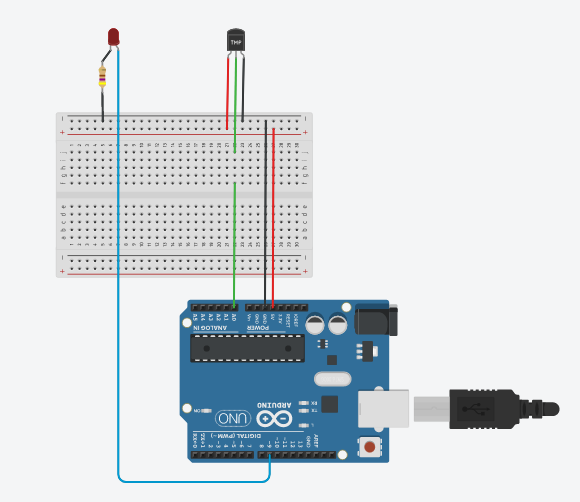
\includegraphics[scale=0.6]{Figures/heat.PNG}
    \caption{Circuit diagram}
\end{figure}

\subsection*{Procedure}
\begin{enumerate}
    \item Copy lst. \ref{lst:temp} to a new Arduino sketchbook. Upload the code to Arduino UNO. Also open the Serial Monitor.
    \item Ask a student to rub their hands and touch the flat side of LM35 module. Observe the change in the readings on the Serial Monitor and in the state of the LED.
\end{enumerate}

\begin{lstlisting}[language=Arduino, numbers=none, caption={Arduino code for measuring the temperature of hands},captionpos=b, label={lst:temp}]

int temp;           // stores the temperature reading 
int tempPin=A0;     // pin A0 reads temperature from temperature sensor
int ledPin=9;       // pin 9 controls the LED
int threshold = 70; // if temperature reading exceeds this threshold, LED will glow

void setup() 
{
  pinMode(tempPin, INPUT);   //configure A0 as input pin
  pinMode(ledPin, OUTPUT);   //configure pin9 as output pin
  Serial.begin(9600);        //set the baud rate to be 9600
  
  digitalWrite(ledPin, LOW); // set pin9 as logic low
 }// void setup ends here

void loop() 
{
  // Measure the temperature reading from pin A0
  temp = analogRead(tempPin);
  
  // Print the temperature reading on the screen
  Serial.println("Temperature= ");
  Serial.print(temp);
  Serial.print(" C");

  // If temperature is greater than the threshold, the LED will glow
  if (temp >= threshold)
    digitalWrite(ledPin, HIGH);
  // ... or else, it will not!
  else
    digitalWrite(ledPin, LOW);
  
  // Wait for 1 sec before the next reading
  delay(1000);
}// loop ends here

\end{lstlisting}

\subsection*{Precautions}
Touch the LM35 module gently. Coarse handling may loosen the connections and affect the measurements.